% !TeX spellcheck = en_GB

\documentclass{beamer}

\usepackage[utf8]{inputenc}
\usepackage[english]{babel}
\usepackage{tabularx}
\usepackage{tikz}
\usepackage{pgfplots}
\usepgfplotslibrary{fillbetween}
\usetikzlibrary{patterns}
\usepackage{xcolor}
\usepackage{listings}

\usetheme{metropolis}

\title{Computer Systems}
\subtitle{Exercises on Models with One Job Class}

\author{Stefano Cereda \\ stefano.cereda@polimi.it}
\date{02/04/2019}
\institute[PoliMi]{\vspace{0.5cm}\centering Politecnico di Milano \\ \vspace{0.2cm}
	\includegraphics[width=0.2\linewidth]{../logopolimi}}
%\logo{\includegraphics[width=15mm]{../logopolimi}}

\setbeamercovered{invisible}

\makeindex

\begin{document}
\begin{frame}
	\maketitle
\end{frame}

\begin{frame}{Disclaimer}
\centering\textbf{\alert{\huge{SKIP THE MVA SECTIONS}}}
\end{frame}

\section{Open models}

\begin{frame}{Recap - Performance bounds}
\centering
$X(\lambda) \leq \frac{1}{D_{max}} \qquad D \leq R(\lambda)$

$\downarrow$

$X(\lambda) \leq \frac{1}{D_{max}} \qquad \frac{D}{1-\lambda D_{avg}} \leq R(\lambda) \leq \frac{D}{1-\lambda D_{max}}$
\end{frame}

\begin{frame}{Open Model Solution Technique}
Processing capacity: $\lambda_{sat}  = \frac{1}{D_{max}}$. We assume $\lambda < \lambda_{sat}$

Throughput: $X(\lambda) = \lambda$

Utilization: $U_k(\lambda) = \lambda D_k$

Residence time: $R_k(\lambda) =
\begin{cases}
	D_k,& \text{for delay centers} \\
	\frac{D_k}{1-U_k(\lambda)},& \text{for queueing centers}
\end{cases}
$

Queue length: $Q_k(\lambda) = \lambda R_k(\lambda) =
\begin{cases}
	U_k(\lambda),& \text{delay} \\
	\frac{U_k(\lambda)}{1-U_K(\lambda)},& \text{queueing}
\end{cases}
$

System response time: $R(\lambda) = \sum_{k=1}^K R_k(\lambda)$

Avg num. in sys.: $Q(\lambda) = \lambda R(\lambda) = \sum_{k=1}^K Q_k(\lambda)$
\end{frame}

\begin{frame}{Exercise 1}
Consider an open system composed by a web server with $D_{ws} = 5ms$, an application server with $D_{as} = 4ms$ and a database with $D_{db} = 3ms$.

Compute and draw throughput and response time bounds, then the tighter ones and compare them with the exact solution.
\end{frame}

\begin{frame}{Solution - performance bounds}
$X(\lambda) \leq \frac{1}{D_{max}} = \frac{1}{0.005} = 200 \qquad 0.012 \leq R(\lambda)$

\vspace{2cm}
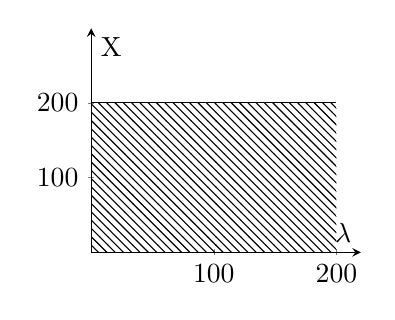
\begin{tikzpicture}[scale = 0.5]
\begin{axis}[
axis y line = left,
axis x line = bottom,
xlabel = $\lambda$,
ylabel = X	,
axis x line=middle,
axis y line=middle,
xtick       = {100,200},
xticklabels = {100,200},
ytick       = {100,200},
yticklabels = {100,200},
samples     = 200,
domain      = 0:200,
xmin = 0, xmax = 220,
ymin = 0, ymax = 300,
]
\addplot[name path=xmax, black,] {200};
\addplot[name path=axis, draw=none] {0};
\addplot[pattern=north west  lines] fill between[of = axis and xmax];
\end{axis}
\end{tikzpicture}
\hspace{1cm}
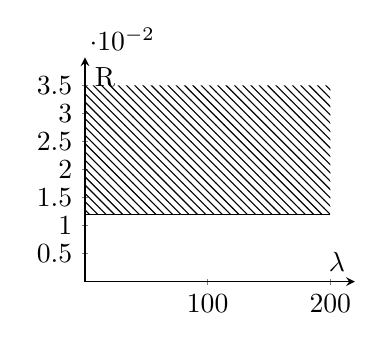
\begin{tikzpicture}[scale = 0.5]
\begin{axis}[
axis y line = left,
axis x line = bottom,
xlabel = $\lambda$,
ylabel = R,
axis x line=middle,
axis y line=middle,
xtick       = {100,200},
xticklabels = {100,200},
ytick       = {0.005, 0.01, 0.015, 0.02, 0.025, 0.03, 0.035, 0.4},
yticklabels = {0.5, 1, 1.5, 2, 2.5, 3, 3.5, 4},
samples     = 200,
domain      = 0:200,
xmin = 0, xmax = 220,
ymin = 0, ymax = 0.04,
]
\addplot[name path=D, black,] {0.012};
\addplot[name path=fake, draw=none] {0.035};
\addplot[pattern=north west  lines] fill between[of = fake and D];
\end{axis}
\end{tikzpicture}

Nearly useless bounds.
\end{frame}

\begin{frame}{Solution - Balanced system bounds}
$X(\lambda) \leq \frac{1}{D_{max}} = \frac{1}{0.005} = 200 \qquad \frac{0.012}{1-\lambda 0.004} \leq R(\lambda) \leq \frac{0.012}{1-\lambda 0.005}$

\vspace{2cm}
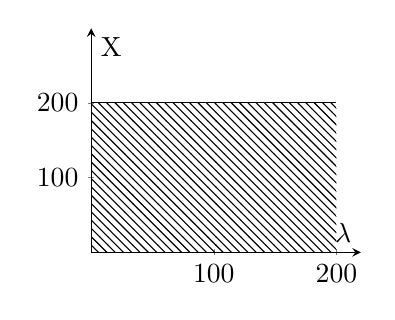
\begin{tikzpicture}[scale = 0.5]
\begin{axis}[
axis y line = left,
axis x line = bottom,
xlabel = $\lambda$,
ylabel = X	,
axis x line=middle,
axis y line=middle,
xtick       = {100,200},
xticklabels = {100,200},
ytick       = {100,200},
yticklabels = {100,200},
samples     = 200,
domain      = 0:200,
xmin = 0, xmax = 220,
ymin = 0, ymax = 300,
]
\addplot[name path=xmax, black,] {200};
\addplot[name path=axis, draw=none] {0};
\addplot[pattern=north west  lines] fill between[of = axis and xmax];
\end{axis}
\end{tikzpicture}
\hspace{1cm}
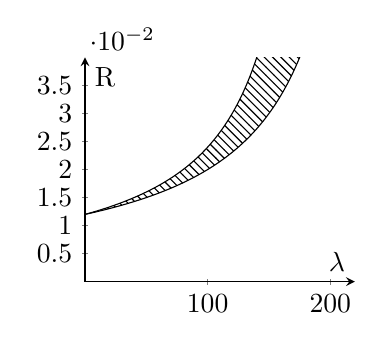
\begin{tikzpicture}[scale = 0.5]
\begin{axis}[
axis y line = left,
axis x line = bottom,
xlabel = $\lambda$,
ylabel = R,
axis x line=middle,
axis y line=middle,
xtick       = {100,200},
xticklabels = {100,200},
ytick       = {0.005, 0.01, 0.015, 0.02, 0.025, 0.03, 0.035, 0.4},
yticklabels = {0.5, 1, 1.5, 2, 2.5, 3, 3.5, 4},
samples     = 200,
domain      = 0:199,
xmin = 0, xmax = 220,
ymin = 0, ymax = 0.04,
]
\addplot[name path=low, black,] {0.012 / (1-0.004*x)};
\addplot[name path=up, black,] {0.012 / (1-0.005*x)};
\addplot[name path=fake, draw=none] {0.02};
\addplot[pattern=north west  lines] fill between[of = up and low];
\end{axis}
\end{tikzpicture}
\end{frame}

\begin{frame}{Solution - Open model solution}
$\lambda < \lambda_{sat} \qquad X(\lambda) = \lambda$ 

$R(\lambda) = \sum R_k(\lambda) \qquad R_k = \frac{D_k}{1-U_k(\lambda)} \qquad U_k(\lambda) = \lambda D_k$

$R(\lambda) = \frac{0.005}{1-\lambda 0.005} + \frac{0.004}{1-\lambda 0.004} + \frac{0.003}{1-\lambda 0.003}$

\begin{tikzpicture}[scale = 0.5]
\begin{axis}[
axis y line = left,
axis x line = bottom,
xlabel = $\lambda$,
ylabel = X	,
axis x line=middle,
axis y line=middle,
xtick       = {100,200},
xticklabels = {100,200},
ytick       = {100,200},
yticklabels = {100,200},
samples     = 200,
domain      = 0:200,
xmin = 0, xmax = 220,
ymin = 0, ymax = 300,
]
\addplot[name path=x, red,] {x};
\end{axis}
\end{tikzpicture}
\hspace{1cm}
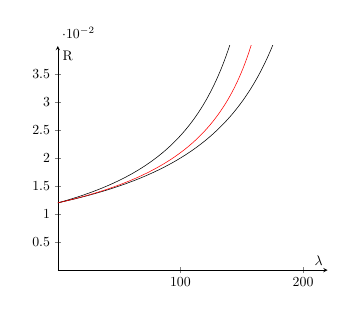
\begin{tikzpicture}[scale = 0.5]
\begin{axis}[
axis y line = left,
axis x line = bottom,
xlabel = $\lambda$,
ylabel = R,
axis x line=middle,
axis y line=middle,
xtick       = {100,200},
xticklabels = {100,200},
ytick       = {0.005, 0.01, 0.015, 0.02, 0.025, 0.03, 0.035, 0.4},
yticklabels = {0.5, 1, 1.5, 2, 2.5, 3, 3.5, 4},
samples     = 200,
domain      = 0:199,
xmin = 0, xmax = 220,
ymin = 0, ymax = 0.04,
]
\addplot[name path=low, black,] {0.012 / (1-0.004*x)};
\addplot[name path=up, black,] {0.012 / (1-0.005*x)};
\addplot[name path=low, red,] {(0.005 / (1-x*0.005)) + (0.004 / (1-x*0.004)) + (0.003 / (1-x*0.003))};
\end{axis}
\end{tikzpicture}
\end{frame}

\begin{frame}{Exercise 2}
$\lambda = 1 \frac{jobs}{sec}$

\vspace{1cm}

\begin{tabular}{ccc}
	$V_{cpu} = 200$	&	$V_{disk1}=50$	&	$V_{disk2} = 30$	\\
	$S_{cpu} = 1ms$	&	$S_{disk1}=10ms$	&	$S_{disk2} = 12ms$	\\
	\hline
	$D_{cpu} = 0.2$	&	$D_{disk1}=0.5$	&	$D_{disk2} = 0.36$	\\
\end{tabular}

\vspace{1cm}

$D_{max} = 0.5 \qquad D=1.06 \qquad D_{avg} = 0.35$
\end{frame}

\begin{frame}{Solution - performance bounds}
$X(\lambda) \leq \frac{1}{D_{max}} = \frac{1}{0.5} = 2 \qquad 1.06 \leq R(\lambda)$

\vspace{2cm}
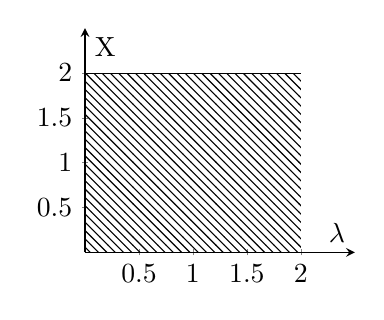
\begin{tikzpicture}[scale = 0.5]
\begin{axis}[
axis y line = left,
axis x line = bottom,
xlabel = $\lambda$,
ylabel = X	,
axis x line=middle,
axis y line=middle,
xtick       = {0.5,1,1.5,2},
xticklabels = {0.5,1,1.5,2},
ytick       = {0.5,1,1.5,2},
yticklabels = {0.5,1,1.5,2},
samples     = 200,
domain      = 0:2,
xmin = 0, xmax = 2.5,
ymin = 0, ymax = 2.5,
]
\addplot[name path=xmax, black,] {2};
\addplot[name path=axis, draw=none] {0};
\addplot[pattern=north west  lines] fill between[of = axis and xmax];
\end{axis}
\end{tikzpicture}
\hspace{1cm}
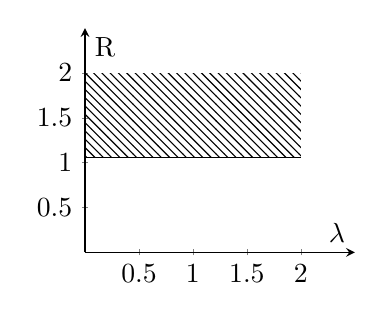
\begin{tikzpicture}[scale = 0.5]
\begin{axis}[
axis y line = left,
axis x line = bottom,
xlabel = $\lambda$,
ylabel = R,
axis x line=middle,
axis y line=middle,
xtick       = {0.5,1,1.5,2},
xticklabels = {0.5,1,1.5,2},
ytick       = {0.5,1,1.5,2},
yticklabels = {0.5,1,1.5,2},
samples     = 200,
domain      = 0:2,
xmin = 0, xmax = 2.5,
ymin = 0, ymax = 2.5,
]
\addplot[name path=D, black,] {1.06};
\addplot[name path=fake, draw=none] {2};
\addplot[pattern=north west  lines] fill between[of = fake and D];
\end{axis}
\end{tikzpicture}
\end{frame}

\begin{frame}{Solution - Balanced system bounds}
$X(\lambda) \leq \frac{1}{D_{max}} = \frac{1}{0.5} = 2 \qquad \frac{1.06}{1-\lambda 0.35} \leq R(\lambda) \leq \frac{1.06}{1-\lambda 0.5}$

\vspace{2cm}
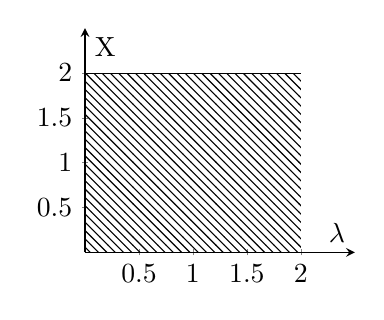
\begin{tikzpicture}[scale = 0.5]
\begin{axis}[
axis y line = left,
axis x line = bottom,
xlabel = $\lambda$,
ylabel = X,
axis x line=middle,
axis y line=middle,
xtick       = {0.5,1,1.5,2},
xticklabels = {0.5,1,1.5,2},
ytick       = {0.5,1,1.5,2},
yticklabels = {0.5,1,1.5,2},
samples     = 200,
domain      = 0:2,
xmin = 0, xmax = 2.5,
ymin = 0, ymax = 2.5,
]
\addplot[name path=xmax, black,] {2};
\addplot[name path=axis, draw=none] {0};
\addplot[pattern=north west  lines] fill between[of = axis and xmax];
\end{axis}
\end{tikzpicture}
\hspace{1cm}
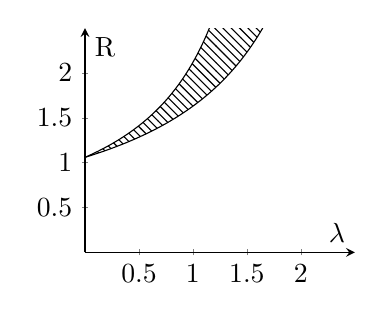
\begin{tikzpicture}[scale = 0.5]
\begin{axis}[
axis y line = left,
axis x line = bottom,
xlabel = $\lambda$,
ylabel = R,
axis x line=middle,
axis y line=middle,
xtick       = {0.5,1,1.5,2},
xticklabels = {0.5,1,1.5,2},
ytick       = {0.5,1,1.5,2},
yticklabels = {0.5,1,1.5,2},
samples     = 200,
domain      = 0:1.9,
xmin = 0, xmax = 2.5,
ymin = 0, ymax = 2.5,
]
\addplot[name path=low, black,] {1.06 / (1-0.35*x)};
\addplot[name path=up, black,] {1.06 / (1-0.5*x)};
\addplot[pattern=north west  lines] fill between[of = up and low];
\end{axis}
\end{tikzpicture}
\end{frame}

\begin{frame}{Some outputs of the model}
$\lambda = 1.5 \frac{jobs}{sec}$

\begin{itemize}
	\item $X_{cpu}(1.5) = \lambda V_{cpu} = 1.5 200 = 300$
	\item $U_{cpu}(1.5) = \lambda D_{cpu} = 1.5 0.2 = 0.3$
	\item $R_{cpu}(1.5) = \frac{D_{cpu}}{1-U_{cpu(1.5)}} = \frac{0.2}{0.7} = 0.286 sec$
	\item $Q_{cpu}(1.5) = \frac{U_{cpu}(1.5)}{1-U_{cpu(1.5)}} = \frac{0.3}{0.7} = 0.428 jobs$
	\item $R(1.5) = R_{cpu}(1.5) + R_{disk1}(1.5) + R_{disk2}(1.5) = 3.068 sec$
	\item $Q(1.5) = \lambda R(1.5) = 4.602 jobs$
\end{itemize}
\end{frame}

\begin{frame}{Solution - Open model solution}
$\lambda < \lambda_{sat} \qquad X(\lambda) = \lambda$ 

$R(\lambda) = \sum R_k(\lambda) \qquad R_k = \frac{D_k}{1-U_k(\lambda)} \qquad U_k(\lambda) = \lambda D_k$

$R(\lambda) = \frac{0.2}{1-\lambda 0.2} + \frac{0.5}{1-\lambda 0.5} + \frac{0.36}{1-\lambda 0.36}$

\begin{tikzpicture}[scale = 0.5]
\begin{axis}[
axis y line = left,
axis x line = bottom,
xlabel = $\lambda$,
ylabel = X,
axis x line=middle,
axis y line=middle,
xtick       = {0.5,1,1.5,2},
xticklabels = {0.5,1,1.5,2},
ytick       = {0.5,1,1.5,2},
yticklabels = {0.5,1,1.5,2},
samples     = 200,
domain      = 0:2,
xmin = 0, xmax = 2.5,
ymin = 0, ymax = 2.5,
]
\addplot[name path=x, red] {x};
\end{axis}
\end{tikzpicture}
\hspace{1cm}
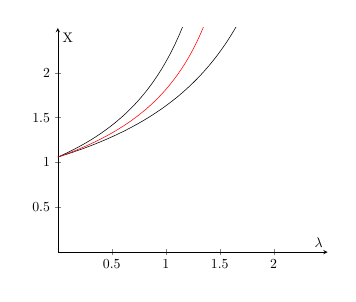
\begin{tikzpicture}[scale = 0.5]
\begin{axis}[
axis y line = left,
axis x line = bottom,
xlabel = $\lambda$,
ylabel = X,
axis x line=middle,
axis y line=middle,
xtick       = {0.5,1,1.5,2},
xticklabels = {0.5,1,1.5,2},
ytick       = {0.5,1,1.5,2},
yticklabels = {0.5,1,1.5,2},
samples     = 200,
domain      = 0:1.9,
xmin = 0, xmax = 2.5,
ymin = 0, ymax = 2.5,
]
\addplot[name path=low, black] {1.06 / (1-0.35*x)};
\addplot[name path=up, black,] {1.06 / (1-0.5*x)};
\addplot[name path=low, red,] {(0.2 / (1-x*0.2)) + (0.5 / (1-x*0.5)) + (0.36 / (1-x*0.36))};
\end{axis}
\end{tikzpicture}
\end{frame}


\section{Closed models - batch workload}
\begin{frame}{Recap - Performance bounds}
\centering
$\frac{1}{D} \leq X(N) \leq \min{(\frac{N}{D}, \frac{1}{D_{max}})} \qquad \max{(D, ND_{max})} \leq R(N) \leq ND$

$\downarrow$

$\frac{N}{D + (N-1)D_{max}} \leq X(N) \leq \min(\frac{1}{D_{max}}, \frac{N}{D + (N-1)D_{avg}})$

$\max(N D_{max}, D + (N-1)D_{avg}) \leq R(N) \leq D + (N-1)D_{max}$

$N^* = D/D_{max} \qquad N^+ = \frac{D-D_{avg}}{D_{max}-D_{avg}}$

The throughput must be computed, the response time is bounded by lines passing through $(1, D)$ and $(0, D-D_{avg}) (0, D-D_{max})$
\end{frame}

\iffalse
\begin{frame}[fragile]{Exact MVA Solution technique}
\lstinputlisting[language=Python, firstline=4, lastline=18, basicstyle=\small]{ex_mva.py}
\end{frame}

\begin{frame}[fragile]{Approximate MVA Solution technique}
\lstinputlisting[language=Python, firstline=4, lastline=20, basicstyle=\small]{appr_mva.py}
\end{frame}
\fi 

\begin{frame}{Exercise 3}
Consider a batch system composed by a web server with $D_{ws} = 5ms$, an application server with $D_{as} = 4ms$ and a database with $D_{db} = 3ms$.

Compute and draw throughput and response time bounds, then the tighter ones and compare them with the exact solution. Then use approximate MVA to compute an estimate of X and R for N=33000.
\end{frame}

\begin{frame}{Solution - performance bounds}
$\frac{1}{0.012} \leq X(n) \leq \min(\frac{N}{0.012}, \frac{1}{0.005}) \qquad$
$\max(0.012, N \cdot 0.005) \leq R(N) \leq N \cdot 0.012$\\
$N^* = \frac{0.012}{0.005} = 2.4$

\vspace{2cm}
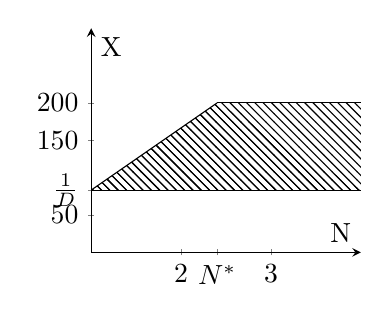
\begin{tikzpicture}[scale = 0.5]
\begin{axis}[
axis y line = left,
axis x line = bottom,
xlabel = N,
ylabel = X	,
axis x line=middle,
axis y line=middle,
xtick       = {1,2,2.4,3},
xticklabels = {1,2,$N^*$,3},
ytick       = {50, 83, 150, 200},
yticklabels = {50, $\frac{1}{D}$, 150, 200},
samples     = 200,
domain      = 1:4,
xmin= 1, xmax = 4,
ymin = 0, ymax = 300,
]
\addplot[name path=low, black,] {1/0.012};
\addplot[name path=up1, black, domain=1:2.4] {x/0.012};
\addplot[name path=up2, black, domain=2.4:4] {1/0.005};
\addplot[pattern=north west lines] fill between[of = low and up1];
\addplot[pattern=north west lines] fill between[of = low and up2];
\end{axis}
\end{tikzpicture}
\hspace{1cm}
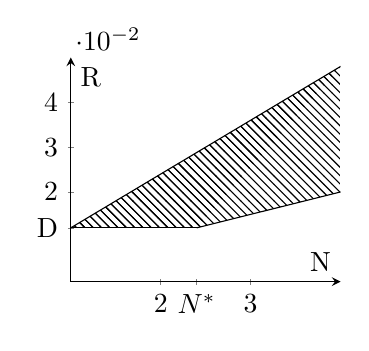
\begin{tikzpicture}[scale = 0.5]
\begin{axis}[
axis y line = left,
axis x line = bottom,
xlabel = N,
ylabel = R,
axis x line=middle,
axis y line=middle,
xtick       = {1,2,2.4,3},
xticklabels = {1,2,$N^*$,3},
ytick       = {0.012, 0.02, 0.03, 0.04},
yticklabels = {D,2,3,4},
samples     = 200,
domain      = 1:4,
xmin= 1, xmax = 4,
ymin = 0, ymax = 0.05,
]
\addplot[name path=low1, black, domain=1:2.4] {0.012};
\addplot[name path=low2, black, domain=2.4:4] {x*0.005};
\addplot[name path=up, black] {x * 0.012};
\addplot[pattern=north west lines] fill between[of = low1 and up];
\addplot[pattern=north west lines] fill between[of = low2 and up];
\end{axis}
\end{tikzpicture}
\end{frame}

\begin{frame}{Solution - Balanced system bounds}
$\frac{N}{0.012 + (N-1)0.005} \leq X(N) \leq \min(\frac{1}{0.005}, \frac{N}{D + (N-1)0.004})$

$\max(N 0.005, D + (N-1)0.004) \leq R(N) \leq D + (N-1)0.005$

$N^+ = \frac{0.012 - 0.004}{0.005 - 0.004} = 8$

\vspace{2cm}
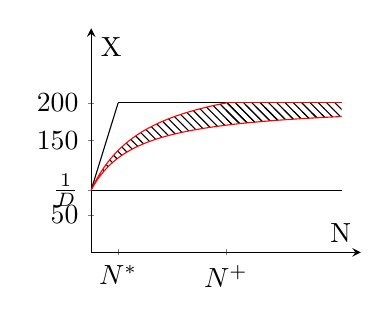
\begin{tikzpicture}[scale = 0.5]
\begin{axis}[
axis y line = left,
axis x line = bottom,
xlabel = N,
ylabel = X	,
axis x line=middle,
axis y line=middle,
xtick       = {1,2.4,8},
xticklabels = {1,$N^*$,$N^+$},
ytick       = {50, 83, 150, 200},
yticklabels = {50, $\frac{1}{D}$, 150, 200},
samples     = 200,
domain      = 1:14,
xmin= 1, xmax = 15,
ymin = 0, ymax = 300,
]
\addplot[name path=low, black,] {1/0.012};
\addplot[name path=up1, black, domain=1:2.4] {x/0.012};
\addplot[name path=up2, black, domain=2.4:14] {1/0.005};
%\addplot[pattern=north west lines] fill between[of = low and up1];
%\addplot[pattern=north west lines] fill between[of = low and up2];

\addplot[name path = tlow, red] {x / (0.012 + (x-1)*0.005)};
\addplot[name path = tup1, red, domain=1:8] {x / (0.012 + (x-1)*0.004)};
\addplot[name path = tup2, red, domain=8:14] {1/0.005};
\addplot[name path = tlow2, draw=none, domain=8:14] {x / (0.012 + (x-1)*0.005)};
\addplot[pattern=north west  lines] fill between[of = tlow and tup1];
\addplot[pattern=north west  lines] fill between[of = tlow2 and tup2];
\end{axis}
\end{tikzpicture}
\hspace{1cm}
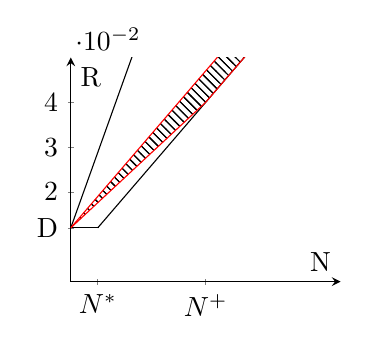
\begin{tikzpicture}[scale = 0.5]
\begin{axis}[
axis y line = left,
axis x line = bottom,
xlabel = N,
ylabel = R,
axis x line=middle,
axis y line=middle,
xtick       = {1,2.4,8},
xticklabels = {1,$N^*$,$N^+$},
ytick       = {0.012, 0.02, 0.03, 0.04},
yticklabels = {D,2,3,4},
samples     = 200,
domain      = 1:14,
xmin= 1, xmax = 15,
ymin = 0, ymax = 0.05,
]
\addplot[name path=low1, black, domain=1:2.4] {0.012};
\addplot[name path=low2, black, domain=2.4:14] {x*0.005};
\addplot[name path=up, black] {x * 0.012};
%\addplot[pattern=north west lines] fill between[of = low1 and up];
%\addplot[pattern=north west lines] fill between[of = low2 and up];

\addplot[name path=tlow2, red, domain=1:8] {0.012+(x-1)*0.004};
\addplot[name path=tlow1, red, domain=8:14] {x*0.005};
\addplot[name path=tup, red] {0.012 + (x-1)*0.005};
\addplot[pattern=north west lines] fill between[of = tlow1 and tup];
\addplot[pattern=north west lines] fill between[of = tlow2 and tup];
\end{axis}
\end{tikzpicture}

Easy to draw.

\end{frame}

\begin{frame}{Solution - Exact MVA}
Use the python code to get N, X, R.

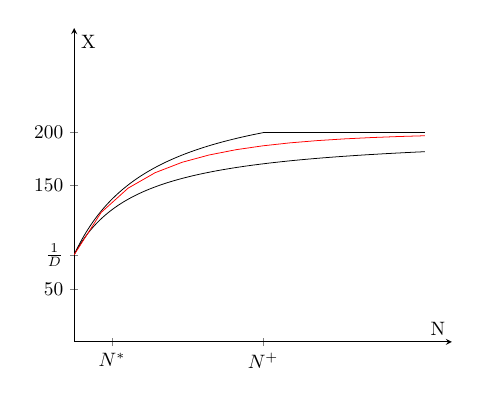
\begin{tikzpicture}[scale = 0.7]
\begin{axis}[
axis y line = left,
axis x line = bottom,
xlabel = N,
ylabel = X	,
axis x line=middle,
axis y line=middle,
xtick       = {1,2.4,8},
xticklabels = {1,$N^*$,$N^+$},
ytick       = {50, 83, 150, 200},
yticklabels = {50, $\frac{1}{D}$, 150, 200},
samples     = 200,
domain      = 1:14,
xmin= 1, xmax = 15,
ymin = 0, ymax = 300,
]
\addplot[name path = tlow, black] {x / (0.012 + (x-1)*0.005)};
\addplot[name path = tup1, black , domain=1:8] {x / (0.012 + (x-1)*0.004)};
\addplot[name path = tup2, black , domain=8:14] {1/0.005};
\addplot [red] coordinates { (1, 83.333333) (2, 123.711340) (3, 146.969697) (4, 161.725067) (5, 171.672556) (6, 178.660273) (7, 183.714412) (8, 187.449483) (9, 190.254965) (10, 192.388780) (11, 194.027726) (12, 195.296391) (13, 196.284549) (14, 197.058080) };
\end{axis}
\end{tikzpicture}
\vspace{1cm}
\begin{tikzpicture}[scale = 0.7]
\begin{axis}[
axis y line = left,
axis x line = bottom,
xlabel = N,
ylabel = R,
axis x line=middle,
axis y line=middle,
xtick       = {1,2.4,8},
xticklabels = {1,$N^*$,$N^+$},
ytick       = {0.012, 0.02, 0.03, 0.04},
yticklabels = {D,2,3,4},
samples     = 200,
domain      = 1:14,
xmin= 1, xmax = 15,
ymin = 0, ymax = 0.05,
]
\addplot[name path=tlow2, black , domain=1:8] {0.012+(x-1)*0.004};
\addplot[name path=tlow1, black , domain=8:14] {x*0.005};
\addplot[name path=tup, black ] {0.012 + (x-1)*0.005};
\addplot [red] coordinates {(1, 0.012000) (2, 0.016167) (3, 0.020412) (4, 0.024733) (5, 0.029125) (6, 0.033583) (7, 0.038103) (8, 0.042678) (9, 0.047305) (10, 0.051978) (11, 0.056693) (12, 0.061445) (13, 0.066230) (14, 0.071045)};
\end{axis}
\end{tikzpicture}
\end{frame}

\begin{frame}{Solution - Approximate MVA}
From exact MVA we know that $X(33000) = 200$ and $R(33000) = 165$

Using 20 iterations of python code for approximate MVA we get:
$X(33000) = 200$ and $R(33000) = 164$

This is a good estimate and requires much less time to be computed.
\end{frame}

\section{Closed models - terminal workloads}

\begin{frame}{Recap - Performance bounds}
\centering
$\frac{N}{ND+Z} \leq X(N) \leq \min{(\frac{N}{D+Z}, \frac{1}{D_{max}})}$\\
$\max{(D, ND_{max} - Z)} \leq R(N) \leq ND$

$\downarrow$

$\frac{N}{D + Z + \frac{(N-1)D_{max}}{1+Z/(ND)}} \leq X(N) \leq \min(\frac{1}{D_{max}}, \frac{N}{D + Z + \frac{(N-1)D_{avg}}{1+Z/D}})$

$\max(N D_{max} - Z, D + \frac{(N-1)D_{avg}}{1+Z/D}) \leq R(N) \leq D + \frac{(N-1)D_{max}}{1+Z/(ND)}$

$N^* = \frac{D+Z}{D_{max}} \qquad N^+ = \frac{(D+Z)^2 -D \cdot D_{avg}}{(D+Z)D_{max} - D\cdot D_{avg}}$

The throughput and the pessimistic bound on response time must be computed.The optimistic bound on response time is a line through the points: $(0, D-\frac{D_{avg}}{1+Z/D})$ and $(1,D)$.

The exact and approximate solutions can be computed as in the previous case.
\end{frame}

\begin{frame}{Exercise 4}
Consider a terminal system composed by a web server with $D_{ws} = 5ms$, an application server with $D_{as} = 4ms$ and a database with $D_{db} = 3ms$. The sleep time is $Z=5s$.

Compute and draw throughput and response time bounds, then the tighter ones and compare them with the exact solution. Then use approximate MVA to compute an estimate of X and R for N=750.
\end{frame}

\begin{frame}{Solution - performance bounds}
$\frac{N}{0.012\cdot N + 5} \leq X(n) \leq \min(\frac{N}{5.012}, \frac{1}{0.005}) \qquad$
$\max(0.012, N \cdot 0.005 - 5) \leq R(N) \leq N \cdot 0.012$\\
$N^* = \frac{5.012}{0.005} = 1002.4$

\vspace{2cm}
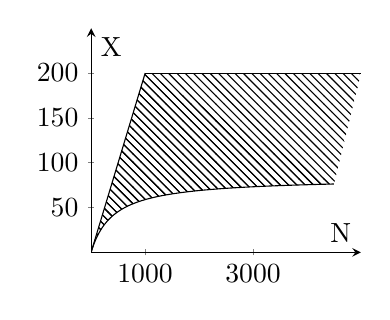
\begin{tikzpicture}[scale = 0.5]
\begin{axis}[
axis y line = left,
axis x line = bottom,
xlabel = N,
ylabel = X	,
axis x line=middle,
axis y line=middle,
xtick       = {1000,3000},
xticklabels = {1000,3000},
ytick       = {50, 100, 150, 200},
yticklabels = {50, 100, 150, 200},
samples     = 200,
domain      = 1:4500,
xmin = 1, xmax = 5000,
ymin = 0, ymax = 250,
]
\addplot[name path=low, black,] {x/(0.012*x +5)};
\addplot[name path=up1, black, domain=1:1002.4] {x/5.012};
\addplot[name path=up2, black, domain=1002.4:5000] {1/0.005};
\addplot[pattern=north west lines] fill between[of = low and up1];
\addplot[pattern=north west lines] fill between[of = low and up2];
\end{axis}
\end{tikzpicture}
\hspace{1cm}
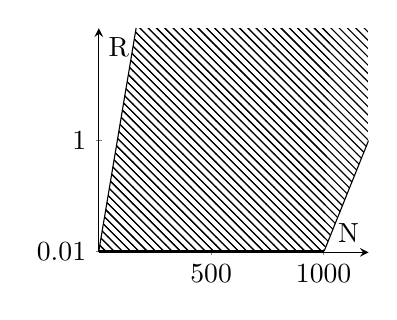
\begin{tikzpicture}[scale = 0.5]
\begin{axis}[
axis y line = left,
axis x line = bottom,
xlabel = N,
ylabel = R,
axis x line=middle,
axis y line=middle,
xtick       = {500, 1000},
xticklabels = {500, 1000},
ytick       = {0.01, 1},
yticklabels = {0.01, 1},
samples     = 200,
domain      = 1:1200,
xmin = 1, xmax = 1200,
ymin = 0, ymax = 2,
]
\addplot[name path=low1, black, domain=1:1002.4] {0.012};
\addplot[name path=low2, black, domain=1002.4:1200] {x*0.005 - 5};
\addplot[name path=up, black] {x * 0.012};
\addplot[pattern=north west lines] fill between[of = low1 and up];
\addplot[pattern=north west lines] fill between[of = low2 and up];
\end{axis}
\end{tikzpicture}
\end{frame}

\begin{frame}{Solution - Balanced system bounds}
$\frac{N}{5.012 + \frac{(N-1)0.005}{1+5/0.012N}} \leq X(N) \leq \min(\frac{1}{0.005}, \frac{N}{5.012 + \frac{(N-1)0.004}{1+5/0.012}})$

$\max(N 0.005 - 5, D + \frac{(N-1)0.004}{1+5/0.012}) \leq R(N) \leq D + \frac{(N-1)0.005}{1+5/0.012N}$

$N^+ = \frac{5.012^2 - 0.012*0.004}{5.012*0.005 - 0.012*0.004} = \frac{25.12}{0.025} = 1004.8$

\vspace{2cm}
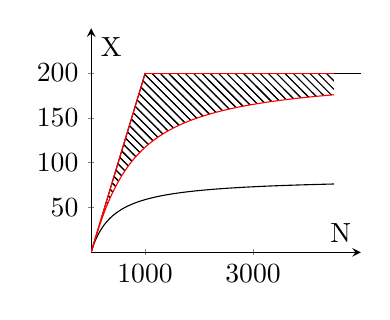
\begin{tikzpicture}[scale = 0.5]
\begin{axis}[
axis y line = left,
axis x line = bottom,
xlabel = N,
ylabel = X	,
axis x line=middle,
axis y line=middle,
xtick       = {1000,3000},
xticklabels = {1000,3000},
ytick       = {50, 100, 150, 200},
yticklabels = {50, 100, 150, 200},
samples     = 200,
domain      = 1:4500,
xmin = 1, xmax = 5000,
ymin = 0, ymax = 250,
]
\addplot[name path=low, black,] {x/(0.012*x +5)};
\addplot[name path=up1, black, domain=1:1002.4] {x/5.012};
\addplot[name path=up2, black, domain=1002.4:5000] {1/0.005};
%\addplot[pattern=north west lines] fill between[of = low and up1];
%\addplot[pattern=north west lines] fill between[of = low and up2];

\addplot[name path=tlow, red] {x / (5.012 + ((x-1)*0.005)/(1+5/(0.012*x))) };
\addplot[name path=tup1, red, domain=1004.8:4500] {1/0.005};
\addplot[name path=tup2, red, domain=1:1004.8] {x / (5.012 + ((x-1)*0.004)/(1+5/(0.012))) };
\addplot[pattern=north west lines] fill between[of = tlow and tup1];
\addplot[pattern=north west lines] fill between[of = tlow and tup2];

\end{axis}
\end{tikzpicture}
\hspace{1cm}
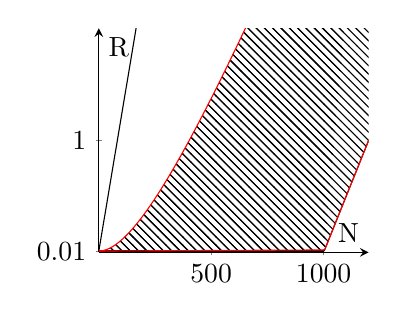
\begin{tikzpicture}[scale = 0.5]
\begin{axis}[
axis y line = left,
axis x line = bottom,
xlabel = N,
ylabel = R,
axis x line=middle,
axis y line=middle,
xtick       = {500, 1000},
xticklabels = {500, 1000},
ytick       = {0.01, 1},
yticklabels = {0.01, 1},
samples     = 200,
domain      = 1:1200,
xmin = 1, xmax = 1200,
ymin = 0, ymax = 2,
]
\addplot[name path=low1, black, domain=1:1002.4] {0.012};
\addplot[name path=low2, black, domain=1002.4:1200] {x*0.005 - 5};
\addplot[name path=up, black] {x * 0.012};
%\addplot[pattern=north west lines] fill between[of = low1 and up];
%\addplot[pattern=north west lines] fill between[of = low2 and up];

\addplot[name path=tlow1, red, domain=1004.8:1500] {x*0.005 - 5};
\addplot[name path=tlow2, red, domain=1:1004.8] {0.012 + ((x-1)*0.004)/(1+5/0.012)};
\addplot[name path=tup, red] {0.012 + ((x-1)*0.005)/(1+5/(0.012*x))};
\addplot[pattern=north west lines] fill between[of = tlow1 and tup];
\addplot[pattern=north west lines] fill between[of = tlow2 and tup];
\end{axis}
\end{tikzpicture}
\end{frame}

\begin{frame}{Solution - Exact MVA}
Use the python code to get N, X, R.

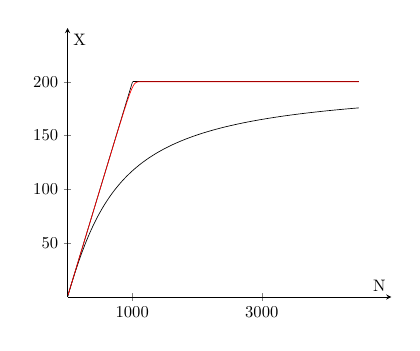
\begin{tikzpicture}[scale = 0.6]
\begin{axis}[
axis y line = left,
axis x line = bottom,
xlabel = N,
ylabel = X	,
axis x line=middle,
axis y line=middle,
xtick       = {1000,3000},
xticklabels = {1000,3000},
ytick       = {50, 100, 150, 200},
yticklabels = {50, 100, 150, 200},
samples     = 200,
domain      = 1:4500,
xmin = 1, xmax = 5000,
ymin = 0, ymax = 250,
]

\addplot[name path=tlow, black] {x / (5.012 + ((x-1)*0.005)/(1+5/(0.012*x))) };
\addplot[name path=tup1, black, domain=1004.8:4500] {1/0.005};
\addplot[name path=tup2, black, domain=1:1004.8] {x / (5.012 + ((x-1)*0.004)/(1+5/(0.012))) };
\addplot [red] coordinates {(10, 1.995176) (20, 3.990270) (30, 5.985280) (40, 7.980206) (50, 9.975043) (60, 11.969789) (70, 13.964443) (80, 15.959002) (90, 17.953462) (100, 19.947822) (110, 21.942077) (120, 23.936226) (130, 25.930266) (140, 27.924192) (150, 29.918001) (160, 31.911690) (170, 33.905256) (180, 35.898694) (190, 37.892000) (200, 39.885171) (210, 41.878202) (220, 43.871088) (230, 45.863825) (240, 47.856407) (250, 49.848830) (260, 51.841087) (270, 53.833174) (280, 55.825084) (290, 57.816812) (300, 59.808349) (310, 61.799690) (320, 63.790827) (330, 65.781753) (340, 67.772459) (350, 69.762937) (360, 71.753178) (370, 73.743173) (380, 75.732911) (390, 77.722382) (400, 79.711574) (410, 81.700477) (420, 83.689077) (430, 85.677361) (440, 87.665316) (450, 89.652925) (460, 91.640173) (470, 93.627043) (480, 95.613517) (490, 97.599575) (500, 99.585196) (510, 101.570360) (520, 103.555040) (530, 105.539213) (540, 107.522850) (550, 109.505922) (560, 111.488397) (570, 113.470241) (580, 115.451416) (590, 117.431881) (600, 119.411594) (610, 121.390505) (620, 123.368564) (630, 125.345712) (640, 127.321889) (650, 129.297025) (660, 131.271045) (670, 133.243866) (680, 135.215398) (690, 137.185537) (700, 139.154172) (710, 141.121176) (720, 143.086409) (730, 145.049712) (740, 147.010907) (750, 148.969793) (760, 150.926141) (770, 152.879690) (780, 154.830144) (790, 156.777158) (800, 158.720337) (810, 160.659222) (820, 162.593276) (830, 164.521870) (840, 166.444261) (850, 168.359568) (860, 170.266738) (870, 172.164504) (880, 174.051336) (890, 175.925369) (900, 177.784317) (910, 179.625363) (920, 181.445012) (930, 183.238908) (940, 185.001602) (950, 186.726269) (960, 188.404368) (970, 190.025268) (980, 191.575889) (990, 193.040458) (1000, 194.400582) (1010, 195.635916) (1020, 196.725797) (1030, 197.652115) (1040, 198.403283) (1050, 198.978365) (1060, 199.389631) (1070, 199.661718) (1080, 199.826949) (1090, 199.918559) (1100, 199.964802) (1110, 199.986036) (1120, 199.994914) (1130, 199.998297) (1140, 199.999476) (1150, 199.999851) (1160, 199.999961) (1170, 199.999991) (1180, 199.999998) (1190, 200.000000) (1200, 200.000000) (1210, 200.000000) (1220, 200.000000) (1230, 200.000000) (1240, 200.000000) (1250, 200.000000) (1260, 200.000000) (1270, 200.000000) (1280, 200.000000) (1290, 200.000000) (1300, 200.000000) (1310, 200.000000) (1320, 200.000000) (1330, 200.000000) (1340, 200.000000) (1350, 200.000000) (1360, 200.000000) (1370, 200.000000) (1380, 200.000000) (1390, 200.000000) (1400, 200.000000) (1410, 200.000000) (1420, 200.000000) (1430, 200.000000) (1440, 200.000000) (1450, 200.000000) (1460, 200.000000) (1470, 200.000000) (1480, 200.000000) (1490, 200.000000) (1500, 200.000000) (1510, 200.000000) (1520, 200.000000) (1530, 200.000000) (1540, 200.000000) (1550, 200.000000) (1560, 200.000000) (1570, 200.000000) (1580, 200.000000) (1590, 200.000000) (1600, 200.000000) (1610, 200.000000) (1620, 200.000000) (1630, 200.000000) (1640, 200.000000) (1650, 200.000000) (1660, 200.000000) (1670, 200.000000) (1680, 200.000000) (1690, 200.000000) (1700, 200.000000) (1710, 200.000000) (1720, 200.000000) (1730, 200.000000) (1740, 200.000000) (1750, 200.000000) (1760, 200.000000) (1770, 200.000000) (1780, 200.000000) (1790, 200.000000) (1800, 200.000000) (1810, 200.000000) (1820, 200.000000) (1830, 200.000000) (1840, 200.000000) (1850, 200.000000) (1860, 200.000000) (1870, 200.000000) (1880, 200.000000) (1890, 200.000000) (1900, 200.000000) (1910, 200.000000) (1920, 200.000000) (1930, 200.000000) (1940, 200.000000) (1950, 200.000000) (1960, 200.000000) (1970, 200.000000) (1980, 200.000000) (1990, 200.000000) (2000, 200.000000) (2010, 200.000000) (2020, 200.000000) (2030, 200.000000) (2040, 200.000000) (2050, 200.000000) (2060, 200.000000) (2070, 200.000000) (2080, 200.000000) (2090, 200.000000) (2100, 200.000000) (2110, 200.000000) (2120, 200.000000) (2130, 200.000000) (2140, 200.000000) (2150, 200.000000) (2160, 200.000000) (2170, 200.000000) (2180, 200.000000) (2190, 200.000000) (2200, 200.000000) (2210, 200.000000) (2220, 200.000000) (2230, 200.000000) (2240, 200.000000) (2250, 200.000000) (2260, 200.000000) (2270, 200.000000) (2280, 200.000000) (2290, 200.000000) (2300, 200.000000) (2310, 200.000000) (2320, 200.000000) (2330, 200.000000) (2340, 200.000000) (2350, 200.000000) (2360, 200.000000) (2370, 200.000000) (2380, 200.000000) (2390, 200.000000) (2400, 200.000000) (2410, 200.000000) (2420, 200.000000) (2430, 200.000000) (2440, 200.000000) (2450, 200.000000) (2460, 200.000000) (2470, 200.000000) (2480, 200.000000) (2490, 200.000000) (2500, 200.000000) (2510, 200.000000) (2520, 200.000000) (2530, 200.000000) (2540, 200.000000) (2550, 200.000000) (2560, 200.000000) (2570, 200.000000) (2580, 200.000000) (2590, 200.000000) (2600, 200.000000) (2610, 200.000000) (2620, 200.000000) (2630, 200.000000) (2640, 200.000000) (2650, 200.000000) (2660, 200.000000) (2670, 200.000000) (2680, 200.000000) (2690, 200.000000) (2700, 200.000000) (2710, 200.000000) (2720, 200.000000) (2730, 200.000000) (2740, 200.000000) (2750, 200.000000) (2760, 200.000000) (2770, 200.000000) (2780, 200.000000) (2790, 200.000000) (2800, 200.000000) (2810, 200.000000) (2820, 200.000000) (2830, 200.000000) (2840, 200.000000) (2850, 200.000000) (2860, 200.000000) (2870, 200.000000) (2880, 200.000000) (2890, 200.000000) (2900, 200.000000) (2910, 200.000000) (2920, 200.000000) (2930, 200.000000) (2940, 200.000000) (2950, 200.000000) (2960, 200.000000) (2970, 200.000000) (2980, 200.000000) (2990, 200.000000) (3000, 200.000000) (3010, 200.000000) (3020, 200.000000) (3030, 200.000000) (3040, 200.000000) (3050, 200.000000) (3060, 200.000000) (3070, 200.000000) (3080, 200.000000) (3090, 200.000000) (3100, 200.000000) (3110, 200.000000) (3120, 200.000000) (3130, 200.000000) (3140, 200.000000) (3150, 200.000000) (3160, 200.000000) (3170, 200.000000) (3180, 200.000000) (3190, 200.000000) (3200, 200.000000) (3210, 200.000000) (3220, 200.000000) (3230, 200.000000) (3240, 200.000000) (3250, 200.000000) (3260, 200.000000) (3270, 200.000000) (3280, 200.000000) (3290, 200.000000) (3300, 200.000000) (3310, 200.000000) (3320, 200.000000) (3330, 200.000000) (3340, 200.000000) (3350, 200.000000) (3360, 200.000000) (3370, 200.000000) (3380, 200.000000) (3390, 200.000000) (3400, 200.000000) (3410, 200.000000) (3420, 200.000000) (3430, 200.000000) (3440, 200.000000) (3450, 200.000000) (3460, 200.000000) (3470, 200.000000) (3480, 200.000000) (3490, 200.000000) (3500, 200.000000) (3510, 200.000000) (3520, 200.000000) (3530, 200.000000) (3540, 200.000000) (3550, 200.000000) (3560, 200.000000) (3570, 200.000000) (3580, 200.000000) (3590, 200.000000) (3600, 200.000000) (3610, 200.000000) (3620, 200.000000) (3630, 200.000000) (3640, 200.000000) (3650, 200.000000) (3660, 200.000000) (3670, 200.000000) (3680, 200.000000) (3690, 200.000000) (3700, 200.000000) (3710, 200.000000) (3720, 200.000000) (3730, 200.000000) (3740, 200.000000) (3750, 200.000000) (3760, 200.000000) (3770, 200.000000) (3780, 200.000000) (3790, 200.000000) (3800, 200.000000) (3810, 200.000000) (3820, 200.000000) (3830, 200.000000) (3840, 200.000000) (3850, 200.000000) (3860, 200.000000) (3870, 200.000000) (3880, 200.000000) (3890, 200.000000) (3900, 200.000000) (3910, 200.000000) (3920, 200.000000) (3930, 200.000000) (3940, 200.000000) (3950, 200.000000) (3960, 200.000000) (3970, 200.000000) (3980, 200.000000) (3990, 200.000000) (4000, 200.000000) (4010, 200.000000) (4020, 200.000000) (4030, 200.000000) (4040, 200.000000) (4050, 200.000000) (4060, 200.000000) (4070, 200.000000) (4080, 200.000000) (4090, 200.000000) (4100, 200.000000) (4110, 200.000000) (4120, 200.000000) (4130, 200.000000) (4140, 200.000000) (4150, 200.000000) (4160, 200.000000) (4170, 200.000000) (4180, 200.000000) (4190, 200.000000) (4200, 200.000000) (4210, 200.000000) (4220, 200.000000) (4230, 200.000000) (4240, 200.000000) (4250, 200.000000) (4260, 200.000000) (4270, 200.000000) (4280, 200.000000) (4290, 200.000000) (4300, 200.000000) (4310, 200.000000) (4320, 200.000000) (4330, 200.000000) (4340, 200.000000) (4350, 200.000000) (4360, 200.000000) (4370, 200.000000) (4380, 200.000000) (4390, 200.000000) (4400, 200.000000) (4410, 200.000000) (4420, 200.000000) (4430, 200.000000) (4440, 200.000000) (4450, 200.000000) (4460, 200.000000) (4470, 200.000000) (4480, 200.000000) (4490, 200.000000) (4500, 200.000000)};
\end{axis}
\end{tikzpicture}
\hspace{1cm}
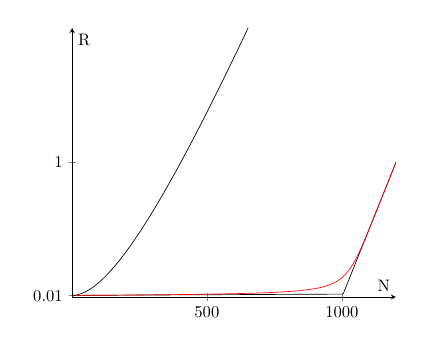
\begin{tikzpicture}[scale = 0.6]
\begin{axis}[
axis y line = left,
axis x line = bottom,
xlabel = N,
ylabel = R,
axis x line=middle,
axis y line=middle,
xtick       = {500, 1000},
xticklabels = {500, 1000},
ytick       = {0.01, 1},
yticklabels = {0.01, 1},
samples     = 200,
domain      = 1:1200,
xmin = 1, xmax = 1200,
ymin = 0, ymax = 2,
]
\addplot[name path=tlow1, black, domain=1004.8:1500] {x*0.005 - 5};
\addplot[name path=tlow2, black, domain=1:1004.8] {0.012 + ((x-1)*0.004)/(1+5/0.012)};
\addplot[name path=tup, black] {0.012 + ((x-1)*0.005)/(1+5/(0.012*x))};
\addplot [red] coordinates {(10, 0.012090) (20, 0.012193) (30, 0.012296) (40, 0.012402) (50, 0.012510) (60, 0.012620) (70, 0.012731) (80, 0.012845) (90, 0.012961) (100, 0.013079) (110, 0.013199) (120, 0.013322) (130, 0.013447) (140, 0.013574) (150, 0.013704) (160, 0.013837) (170, 0.013972) (180, 0.014110) (190, 0.014251) (200, 0.014395) (210, 0.014542) (220, 0.014692) (230, 0.014846) (240, 0.015002) (250, 0.015163) (260, 0.015327) (270, 0.015495) (280, 0.015666) (290, 0.015842) (300, 0.016022) (310, 0.016206) (320, 0.016395) (330, 0.016589) (340, 0.016787) (350, 0.016991) (360, 0.017199) (370, 0.017414) (380, 0.017634) (390, 0.017860) (400, 0.018092) (410, 0.018331) (420, 0.018576) (430, 0.018829) (440, 0.019089) (450, 0.019357) (460, 0.019633) (470, 0.019917) (480, 0.020211) (490, 0.020514) (500, 0.020827) (510, 0.021150) (520, 0.021484) (530, 0.021830) (540, 0.022188) (550, 0.022559) (560, 0.022944) (570, 0.023344) (580, 0.023758) (590, 0.024189) (600, 0.024638) (610, 0.025105) (620, 0.025591) (630, 0.026099) (640, 0.026630) (650, 0.027185) (660, 0.027765) (670, 0.028374) (680, 0.029013) (690, 0.029685) (700, 0.030392) (710, 0.031137) (720, 0.031924) (730, 0.032757) (740, 0.033640) (750, 0.034578) (760, 0.035576) (770, 0.036640) (780, 0.037779) (790, 0.038999) (800, 0.040312) (810, 0.041727) (820, 0.043259) (830, 0.044922) (840, 0.046735) (850, 0.048718) (860, 0.050898) (870, 0.053306) (880, 0.055980) (890, 0.058963) (900, 0.062314) (910, 0.066100) (920, 0.070407) (930, 0.075341) (940, 0.081037) (950, 0.087661) (960, 0.095423) (970, 0.104584) (980, 0.115466) (990, 0.128459) (1000, 0.144018) (1010, 0.162651) (1020, 0.184882) (1030, 0.211176) (1040, 0.241849) (1050, 0.276956) (1060, 0.316224) (1070, 0.359064) (1080, 0.404676) (1090, 0.452220) (1100, 0.500968) (1110, 0.550388) (1120, 0.600142) (1130, 0.650048) (1140, 0.700015) (1150, 0.750004) (1160, 0.800001) (1170, 0.850000) (1180, 0.900000) (1190, 0.950000) (1200, 1.000000) (1210, 1.050000) (1220, 1.100000) (1230, 1.150000) (1240, 1.200000) (1250, 1.250000) (1260, 1.300000) (1270, 1.350000) (1280, 1.400000) (1290, 1.450000) (1300, 1.500000) (1310, 1.550000) (1320, 1.600000) (1330, 1.650000) (1340, 1.700000) (1350, 1.750000) (1360, 1.800000) (1370, 1.850000) (1380, 1.900000) (1390, 1.950000) (1400, 2.000000) (1410, 2.050000) (1420, 2.100000) (1430, 2.150000) (1440, 2.200000) (1450, 2.250000) (1460, 2.300000) (1470, 2.350000) (1480, 2.400000) (1490, 2.450000) (1500, 2.500000) };
\end{axis}
\end{tikzpicture}
\end{frame}

\begin{frame}{Solution - Approximate MVA}
From exact MVA we know that $X(750) = 148.97$ and $R(750) = 0.035$

Using 15 iterations of python code for approximate MVA we get:
$X(750) = 148.75$ and $R(750) = 0.042$
\end{frame}

\end{document}
